%* Source: https://tex.stackexchange.com/a/158979
\documentclass[tikz]{standalone}
\usepackage{pgfplots, calc, tkz-euclide}
\pgfplotsset{compat=1.18}
\usetikzlibrary{decorations.pathreplacing, decorations.markings, angles}

% axis style, ticks, etc
\pgfplotsset{every axis/.append style={
                    axis x line=middle,    % put the x axis in the middle
                    axis y line=middle,    % put the y axis in the middle
                    axis line style={->}, % arrows on the axis
                    xlabel={\(x\)},          % default put x on x-axis
                    ylabel={\(y\)},          % default put y on y-axis
                    axis line style = thick,
                    }}

% arrows as stealth fighters
\tikzset{>=stealth,
-<-/.style={decoration={
  markings,
  mark=at position #1 with {\arrow[scale=1.5]{Classical TikZ Rightarrow[reversed]}}},postaction={decorate}}}
\NewDocumentCommand\bisector{O{}mmmO{10pt}}{
\path[#1] let
    \p1 = ($(#3)!10cm!(#2)$),
    \p2 = ($(#3)!10cm!(#4)$),
    \p3 = ($(\p1) + (\p2) - (#3)$)
    in    
    ($(#3)!#5!($(#3)!0.85cm!(\p3)$)$) -- ($($(#3)!0.85cm!(\p3)$)!#5!(#3)$) ;
}
\begin{document}

\begin{tikzpicture}[
    dot/.style={draw,fill,circle,inner sep=1.7pt,thick},
    odot/.style={draw,circle,inner sep=1pt,thick}]
    \def\a{0.6}
    \def\b{1} 
    \begin{axis}[
        xmin=-0.5,xmax=4.5,
        ymin=-0.5,ymax=4.5,
        ticks=none]
        % Parabolic pdf
        \addplot [blue,thick,domain=0:4.2] {\a*x+\b};
        % Points
        \coordinate[dot,blue] (P1) at (axis cs:1,2) {};
        \coordinate[dot,blue] (P2) at (axis cs:2,1) {};
        \coordinate[dot,blue] (P3) at (axis cs:3,4) {};
        \coordinate[dot,blue] (P4) at (axis cs:4,3) {};
        \coordinate (V1) at (axis cs:1,1.6) {};
        \coordinate (V2) at (axis cs:2,2.2) {};
        \coordinate (V3) at (axis cs:3,2.8) {};
        \coordinate (V4) at (axis cs:4,3.4) {};
        % Error bars
        \draw[dashed,thick,red] (P1) -- (V1) node [midway,left] {\(e_1\)};
        \draw[dashed,thick,red] (P2) -- (V2) node [midway,left] {\(e_2\)};
        \draw[dashed,thick,red] (P3) -- (V3) node [midway,left] {\(e_3\)};
        \draw[dashed,thick,red] (P4) -- (V4) node [midway,below left] {\(e_4\)};
    \end{axis}
\end{tikzpicture}
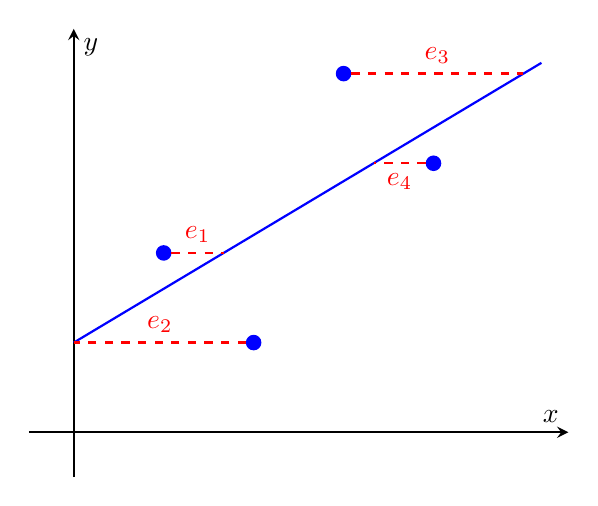
\begin{tikzpicture}[
    dot/.style={draw,fill,circle,inner sep=1.7pt,thick},
    odot/.style={draw,circle,inner sep=1pt,thick}]
    \def\a{0.6}
    \def\b{1} 
    \begin{axis}[
        xmin=-0.5,xmax=5.5,
        ymin=-0.5,ymax=4.5,
        ticks=none]
        % Parabolic pdf
        \addplot [blue,thick,domain=0:5.2] {\a*x+\b};
        % Points
        \coordinate[dot,blue] (P1) at (axis cs:1,2) {};
        \coordinate[dot,blue] (P2) at (axis cs:2,1) {};
        \coordinate[dot,blue] (P3) at (axis cs:3,4) {};
        \coordinate[dot,blue] (P4) at (axis cs:4,3) {};
        \coordinate (V1) at (axis cs:5/3,2) {};
        \coordinate (V2) at (axis cs:0,1) {};
        \coordinate (V3) at (axis cs:5,4) {};
        \coordinate (V4) at (axis cs:10/3,3) {};
        % Error bars
        \draw[dashed,thick,red] (P1) -- (V1) node [midway,above] {\(e_1\)};
        \draw[dashed,thick,red] (P2) -- (V2) node [midway,above] {\(e_2\)};
        \draw[dashed,thick,red] (P3) -- (V3) node [midway,above] {\(e_3\)};
        \draw[dashed,thick,red] (P4) -- (V4) node [midway,below] {\(e_4\)};
    \end{axis}
\end{tikzpicture}
\begin{tikzpicture}[
    dot/.style={draw,fill,circle,inner sep=1.7pt,thick},
    odot/.style={draw,circle,inner sep=1pt,thick}]
    \def\a{0.6}
    \def\b{1} 
    \begin{axis}[
        xmin=-0.5,xmax=4.5,
        ymin=-0.5,ymax=4.5,
        ticks=none]
        % Parabolic pdf
        \addplot [blue,thick,domain=0:4.2] {\a*x+\b};
        % Points
        \coordinate[dot,blue] (P1) at (axis cs:1,2) {};
        \coordinate[dot,blue] (P2) at (axis cs:2,1) {};
        \coordinate[dot,blue] (P3) at (axis cs:3,4) {};
        \coordinate[dot,blue] (P4) at (axis cs:4,3) {};
        \coordinate (V1) at (axis cs:1,1.6) {};
        \coordinate (V2) at (axis cs:2,2.2) {};
        \coordinate (V3) at (axis cs:3,2.8) {};
        \coordinate (V4) at (axis cs:4,3.4) {};
        % Error bars
        \draw[dashed,thick,red] (P1) -- (V1);
        \draw[dashed,thick,red] (P2) -- (V2);
        \draw[dashed,thick,red] (P3) -- (V3) ;
        \draw[dashed,thick,red] (P4) -- (V4);
    \end{axis}
\end{tikzpicture}
\end{document}